%%%%%%%%%%%%%%%%%%%%%%%%%%%%%%%%%%%%%%%%%
% TMDEI Dissertation
% LaTeX Template
% Version 0.1 (Dec/2015)
%
% Adapted to TMDEI/ISEP style (Dec/2015) by
%  Nuno Pereira (nap@isep.ipp.pt) and
%  Paulo Baltarejo (pbs@isep.ipp.pt)
%
% Based on MastersDoctoralThesis Version 1.2 by Vel (vel@latextemplates.com) and
% Johannes Böttcher, downloaded from (21/11/15):
% http://www.LaTeXTemplates.com
%
% This template is originally based on a template by:
% Steve Gunn (http://users.ecs.soton.ac.uk/srg/softwaretools/document/templates/)
% Sunil Patel (http://www.sunilpatel.co.uk/thesis-template/)
%
% Template license:
% CC BY-NC-SA 3.0 (http://creativecommons.org/licenses/by-nc-sa/3.0/)
%
%%%%%%%%%%%%%%%%%%%%%%%%%%%%%%%%%%%%%%%%%
%https://www.overleaf.com/project/5bfd7e508cfbf932785021c9
%----------------------------------------------------------------------------------------
%	PACKAGES AND OTHER DOCUMENT CONFIGURATIONS
%----------------------------------------------------------------------------------------

\documentclass[
11pt, % The default document font size, options: 10pt, 11pt, 12pt
%oneside, % Two side (alternating margins) for binding by default, uncomment to switch to one side (for drafting/reading purposes)
english, % english for English;
%portuguese,% for Portuguese; delete temporary files if you change language (e.g. 'make clean; make')
singlespacing, % Single line spacing, alternatives: onehalfspacing or doublespacing (for drafting/reading purposes)
%draft, % Uncomment to enable draft mode (no pictures, no links, overfull hboxes indicated)
%nolistspacing, % If the document is onehalfspacing or doublespacing, uncomment this to set spacing in lists to single
liststotoc, % Uncomment to add the list of figures/tables/etc to the table of contents (not recommended)
%toctotoc, % Uncomment to add the main table of contents to the table of contents (not recommended)
parskip, % Add space between paragraphs (recommended)
%nohyperref, % Uncomment to not load the hyperref package (not recommended)
nohyperreflinkcolor, % hyperref links are not colored (comment to color links, for example to produce an electronic-only version)
headsepline, % Uncomment to get a line under the header
]{tmdei-style} % The class file specifying the document structure

\usepackage{tikz} % Required for creating graphics programmatically (can be removed if not used)
%\usetikzlibrary{arrows} % Required for fancy arrows in TiKZ graphics (can be removed if not used)

\usepackage{pgfplots} % Required for drawing high--quality function plots (can be removed if not used)
\pgfplotsset{compat=newest}

%
% Next you have examples of admissable citation styles; we recomend using the authoryear-comp citation style (which resembles Harvard); don't forget to only uncomment one
%

% authoryear-comp: recommended citation style (e.g. (Buendía, 1860), (Buendía 1910, Arcadio 1940))
\usepackage[style=authoryear-comp,backend=biber]{biblatex} % Bibtex backend with the authoryear-comp citation style (authoryear citations, bibliography ordered alphabetically)

% numeric citation style (e.g. [1], [1-3])
%\usepackage[style=numeric-comp,sorting=none,backend=biber]{biblatex} % Bibtex backend with the numeric-comp citation style (numeric citations, bibliography ordered by appearance)

% alphabetic citation style (e.g. [Buendía10], [Buendía10, Arcadio40])
%\usepackage[style=alphabetic,sorting=none,backend=biber]{biblatex} % Bibtex backend with the alphabetic citation style (alphabetic citations, bibliography ordered by appearance)


\addbibresource{mainbibliography.bib} % The filename of the bibliography

\makeglossaries % build the glossary

%----------------------------------------------------------------------------------------
%	THESIS INFORMATION
%----------------------------------------------------------------------------------------

\thesistitle{Smart IoT Service Builder Platform} % Your thesis title, this is used in the title, print it elsewhere with \ttitle

%\thesissubtitle{{[}Thesis Subtitle{]}} % Your thesis title, this is used in the title, print it elsewhere with \tsubtitle

\author{Filipe \textsc{Cruz}} % Your name, this is used in the title page, print it elsewhere with \authorname

\subjectarea{Software Engineering} % Specialisation area (Computer Systems, Information and Knowledge Systems, Graphics, Systems and Multimedia, Software Engineering), used in the title page, print it elsewhere with \areaname

\supervisor{Dr. Nuno \textsc{Silva}} % Your supervisor's name, this is used in the title page, print it elsewhere with \supname

%\cosupervisor{Dr. Jack \textsc{Smith}} % Your co-supervisor's name, this is used in the title page, print it elsewhere with \cosupname (comment, if no co-supervisor)

\committeepresident{TODO, Professor, DEI/ISEP} % Name of the president of the evaluation committee, print it elsewhere with \presidentname

\committeemembers{TODO, Professor, DEI/ISEP\\TODO, Professor, DEI/ISEP\\TODO, Professor, DEI/ISEP} % Name of the evaluation committee members (up to four), print it elsewhere with \committee

\keywords{Internet of Things, Stream Processing, Big Data, Configurability, Real Time Systems} % Please define up to 6 keywords that better describe your work, print it elsewhere with \keywordnames

\university{\href{https://www.isep.ipp.pt/}{ISEP}} % Your university's name and URL, this is used in the title page and abstract, print it elsewhere with \univname

\department{\href{https://www.dei.isep.ipp.pt/}{DEI}} % Your department's name and URL, this is used in the title page and abstract, print it elsewhere with \deptname

\thesisdate{Porto, \today} % thesis date,  print it elsewhere with \tdate

\hypersetup{pdftitle=\ttitle} % Set the PDF's title to your title
\hypersetup{pdfauthor=\authorname} % Set the PDF's author to your name
\hypersetup{pdfkeywords=\keywordnames} % Set the PDF's keywords to your keywords

\begin{document}

%----------------------------------------------------------------------------------------
%	FRONT MATTER
%----------------------------------------------------------------------------------------

% Include the frontmatter of your thesis here
%All acronyms must be written in this file.
\newacronym{RTS}{RTS}{Real-Time System}
\newacronym{IoT}{IoT}{Internet of Things}
\newacronym{ETL}{ETL}{Extract, Transform, Load}
\newacronym{GPS}{GPS}{Global Positioning System}
\newacronym{MVP}{MVP}{Minimal Value Product}
\newacronym{UML}{UML}{Unified Modeling Language}
\newacronym{DBMS}{DBMS}{Database Management System}
\newacronym{UI}{UI}{User Interface}
\newacronym{SDK}{SDK}{Software Development Kit}
\newacronym{SRP}{SRP}{Single Responsability Principle}
\newacronym{DIP}{DIP}{Dependency Inversion Principle}
\newacronym{CIAM}{CIAM}{Customer Identity and Access Management}
\newacronym{SOA}{SOA}{Service Oriented Architecture}
\newacronym{ESB}{ESB}{Enterprise Service Bus}


\frontmatter % Use roman page numbering style (i, ii, iii, iv...) for the pre-content pages

\pagestyle{plain} % Default to the plain heading style until the thesis style is called for the body content

%----------------------------------------------------------------------------------------
%	TITLE PAGE
%----------------------------------------------------------------------------------------

\maketitlepage

\clearpage

\thispagestyle{empty}
\null\vfill

\settowidth\longest{\huge\itshape Experience is merely the name}
\centering
\parbox{\longest}{%
  \raggedright{\huge\itshape%
   Experience is merely the name \\ 
   men gave to their mistakes.\par\bigskip
  }   
  \raggedleft\Large\MakeUppercase{Oscar Wilde}\par%
}

\vfill\vfill

\clearpage
\raggedright
%----------------------------------------------------------------------------------------
%	DEDICATION  (optional)
%----------------------------------------------------------------------------------------
%
%\dedicatory{For/Dedicated to/To my\ldots}
\begin{dedicatory}

TODO

\end{dedicatory}

%----------------------------------------------------------------------------------------
%	ABSTRACT PAGE
%----------------------------------------------------------------------------------------

\begin{abstract}

% here you put the abstract in the main language of the work.

Today there are more smart devices than people. The number of devices worldwide is forecast to almost triple from 8.74 billion in 2020 to more than 25.4 billion devices in 2030.

The \gls{IoT} is the connection of millions of smart devices and sensors connected to the Internet. These connected devices and sensors collect and share data for use and analysis by many organizations.
Some examples of intelligent connected sensors are: GPS asset tracking, parking spots, refrigerator thermostats, soil condition and many others. The limit of different objects that could become intelligent sensors is limited only by our imagination. But this devices are mostly useless without a platform to analyze, store and present the aggregated data.

Recently, several platforms have emerged to address this need and help companies/governments to increase efficiency, cut on operational costs and improve safety. Sadly, most of this platforms are tailor made for the devices that the company offers. This dissertation presents a platform focused on enabling other to create \gls{IoT}-based services and three \gls{PoC} services built on top of this platform. This platform attempts to be device-neutral, \gls{IoT} middleware-neutral and provide flexible upstream integration and hosting options while providing a simple and concise data streaming \gls{API}. 

\end{abstract}

\begin{abstractotherlanguage}
% here you put the abstract in the "other language": English, if the work is written in Portuguese; Portuguese, if the work is written in English.

Atualmente, existem mais sensores inteligentes do que pessoas. O número de sensores em todo o mundo deve quase triplicar de 8,74 bilhões em 2020 para mais de 25,4 bilhões em 2030.

O conceito de \gls{IoT} está relacionado com a interação entre milhões de dispositivos inteligentes através da Internet. Estes dispositivos e sensores conectados recolhem e disponibilizam dados para uso e análise por parte de muitas organizações.
Alguns exemplos de sensores inteligentes e seus usos são: dispositivos GPS para rastreamento de ativos, monitorização de vagas de estacionamento, termostatos em arcas frigoríficas, condição do solo e muitos outros. O número de diferentes objetos que podem vir-se a tornar sensores inteligentes é limitado apenas pela nossa imaginação. Mas estes dispositivos são praticamente inúteis sem uma plataforma para analisar, armazenar e apresentar os dados por eles agregados.

Recentemente, várias plataformas surgiram para responder a essa necessidade e ajudar empresas/governos a aumentar a sua eficiência, reduzir custos operacionais e melhorar a segurança dos espaços e negócios. Infelizmente, a maioria dessas plataformas é feita à medida para os dispositivos que a empresa em questão oferece. Esta tese apresenta uma plataforma focada em que propiciar a criação de serviços relacionados com \gls{IoT} e três provas de conceito apoiadas pela plataforma em questão. Esta plataforma procura ser agnóstica em relação aos dispositivos inteligentes e middleware de \gls{IoT} usados por terceiros, oferece variadas e flexíveis opções de integração e hosting como também uma \gls{API} de streaming simples e concisa.

\end{abstractotherlanguage}

%----------------------------------------------------------------------------------------
%	ACKNOWLEDGEMENTS (optional)
%----------------------------------------------------------------------------------------

\begin{acknowledgements}
The completion of this undertaking could not have been possible without the never ending support of those close to me. 

First of all, i would like to thank Professor Dr. Nuno Silva for the involvement and support manifested during this project and my scholarship. 
I would like to express a deep appreciation and indebtedness to all my close relatives and friends that helped me turn this dream into a reality.
Lastly, i would like to thank Margarida for making this journey bearable.

Thank you
\end{acknowledgements}

%----------------------------------------------------------------------------------------
%	LIST OF CONTENTS/FIGURES/TABLES PAGES
%----------------------------------------------------------------------------------------

\tableofcontents % Prints the main table of contents

\listoffigures % Prints the list of figures

\listoftables % Prints the list of tables

%\iflanguage{portuguese}{
%\renewcommand{\listalgorithmname}{Lista de Algor\'itmos}
%}
%\listofalgorithms % Prints the list of algorithms
%\addchaptertocentry{\listalgorithmname}


\renewcommand{\lstlistlistingname}{List of Source Code}
\iflanguage{portuguese}{
\renewcommand{\lstlistlistingname}{Lista de C\'odigo}
}
\lstlistoflistings % Prints the list of listings (programming language source code)
\addchaptertocentry{\lstlistlistingname}


%----------------------------------------------------------------------------------------
%	ABBREVIATIONS
%----------------------------------------------------------------------------------------
%\begin{abbreviations}{ll} % Include a list of abbreviations (a table of two columns)
%%\textbf{LAH} & \textbf{L}ist \textbf{A}breviations \textbf{H}ere\\
%%\textbf{WSF} & \textbf{W}hat (it) \textbf{S}tands \textbf{F}or\\
%\end{abbreviations}

%----------------------------------------------------------------------------------------
%	SYMBOLS
%----------------------------------------------------------------------------------------

%\begin{symbols}{lll} % Include a list of Symbols (a three column table)

%$a$ & distance & \si{\meter} \\
%$P$ & power & \si{\watt} (\si{\joule\per\second}) \\
%Symbol & Name & Unit \\

%\addlinespace % Gap to separate the Roman symbols from the Greek

%$\omega$ & angular frequency & \si{\radian} \\

%\end{symbols}



%----------------------------------------------------------------------------------------
%	ACRONYMS
%----------------------------------------------------------------------------------------

\newcommand{\listacronymname}{List of Acronyms}
\iflanguage{portuguese}{
\renewcommand{\listacronymname}{Lista de Acr\'onimos}
}

%Use GLS
\glsresetall
\printglossary[title=\listacronymname,type=\acronymtype,style=long]

%----------------------------------------------------------------------------------------
%	DONE
%----------------------------------------------------------------------------------------

\mainmatter % Begin numeric (1,2,3...) page numbering
\pagestyle{thesis} % Return the page headers back to the "thesis" style


%----------------------------------------------------------------------------------------
%	MAIN BODY
%----------------------------------------------------------------------------------------

% Include the chapters of the thesis as separate folder for each chapter
% Uncomment the lines as you write the chapters

% Chapter 1
% 
\chapter{Introduction} % Main chapter title
\label{chap:Chapter1} % For referencing the chapter elsewhere, use Chapter~\ref{Chapter1}


%-------------------------------------------------------------------------------
%---------
%
\section{Problem}
\label{sec:problem}

\section{Context}
\label{sec:context}

\section{Approach}
\label{sec:approach}

\section{Objectives}
\label{sec:Oõbjectives}

\section{Achieved Results}
\label{sec:achieved_results}

\section{Document Structure}
\label{sec:document_structure}

% Chapter 2

\chapter{State of the Art} % Main chapter title
\label{chap:Chapter2} % For referencing the chapter elsewhere, use \ref{chap:Chapter2} 

%----------------------------------------------------------------------------------------

\section{Internet of Things}

\subsection{Brief Description}

\subsection{Practical Applications}

\subsection{Enterprise Challenges}

\subsection{Renowned Solutions}

\section{Big Data}

\subsection{Brief Description}

\subsection{Challenges}

\section{Synopsis}
% Chapter 3

\chapter{Analysis} % Main chapter title

\label{chap:Chapter3} % For referencing the chapter elsewhere, use \ref{chap:Chapter3} 

%----------------------------------------------------------------------------------------

\section{Business Analysis}

\subsection{Fleet Management}

\subsection{Smart Irrigation}

\subsection{Asset Tracking}

\subsection{Smart Parking}

\subsection{Public Health and Indoor Fire Outbreak Surveillance}

\section{Technical Analysis}

\subsection{Data Aggregation}

\subsection{Data Filtering}

\subsection{Data Storage}

\subsection{Data Transformation}

\subsection{Data Analysis}

\subsection{Data Presentation}

\subsection{Trigger Warning System}

\subsection{User Authentication/Authorisation}

\section{Synopsis}
% Chapter 4

\chapter{Requirements Elicitation} % Main chapter title

\label{chap:Chapter4} % For referencing the chapter elsewhere, use \ref{chap:Chapter4} 

%----------------------------------------------------------------------------------------

\section{Functional Requirements}

\section{Non Functional Requirements}

\section{Synopsis}
% Chapter 6

\chapter{Design - Environment} % Main chapter title

\label{chap:Chapter6} % For referencing the chapter elsewhere, use \ref{chap:Chapter6} 

%----------------------------------------------------------------------------------------

\section{Reference architecture}

\section{Shared Domain}

\section{Configuration View}

\section{Operation View}

\section{C4 Level 1 - Context}

\section{C4 Level 2 - Containers}

\section{C4 Level 3 - Components}

\section{Synopsis}
% Chapter 7

\chapter{Implementation} % Main chapter title

\label{chap:Chapter7} % For referencing the chapter elsewhere, use \ref{chap:Chapter7} 

%----------------------------------------------------------------------------------------

\section{Technical Environment Decisions}

\section{Technical Environment Description}

\section{Environment Testing}

\section{Synopsis}
% Chapter 8

\chapter{Evaluation of the Solution} % Main chapter title

\label{chap:Chapter8} % For referencing the chapter elsewhere, use \ref{chap:Chapter8} 

%----------------------------------------------------------------------------------------

\section{Approach}

\section{Subjective Critique Evaluation - Configuration View}

\section{Subjective Critique Evaluation - Operation View}

\section{Synopsis}
% Chapter 9

\chapter{Conclusion} % Main chapter title

\label{chap:Chapter9} % For referencing the chapter elsewhere, use \ref{chap:Chapter9} 

%----------------------------------------------------------------------------------------

\section{Achievements}

\section{Unachieved Results}

\section{Future Work}

\section{Synopsis}


%----------------------------------------------------------------------------------------
%	BIBLIOGRAPHY
%----------------------------------------------------------------------------------------

\printbibliography[heading=bibintoc]

%----------------------------------------------------------------------------------------
%	THESIS CONTENT - APPENDICES
%----------------------------------------------------------------------------------------

\appendix % Cue to tell LaTeX that the following "chapters" are Appendices

% Include the appendices of the thesis as separate files from the Appendices folder
% Uncomment the lines as you write the Appendices

\chapter{Data Unit - Shared Model Schema}
\label{AppendixA}

This schema represents the Shared Model Schema of a Data Unit as of \textit{iot-core} package version \textit{0.1.20}.

Due to the lack of standards, this model and the represented measures are possibly incomplete. As the \gls{IoT} landscape evolves and defines stricter and well-known standards for sensor measurements and device parameters representation, the \textit{iot-core} package must adhere to them and be able to translate between the supported representations.

The version that is currently in development, \textit{0.2.0}, is planed to support \citetitle{RFC8428}. The reason behind the delayed support for it, steams from the lack of open-source \textit{Java} libraries related to \textit{SenML}, the unfamiliarity of the author with the standard till early April 2022, and the fast paced development of the solution required to meet costumers' needs. 

\begin{lstlisting}[style=json, caption=Data Unit - Shared Model Schema, label={code:AppendixA:schema}]
{
  "dataId": "[uuid]",
  "reportedAt": "[long]",
  "device": {
    "id": "[uuid]",
    "name": "[string]",
    "downlink": "[string]",
    "records": [{
      "label": "[string]",
      "content": "[string]"
    }],
    "domains":  ["[uuid]"],
    "commands": {
      "[int]": [{
        "id": "[uuid]",
        "name": "[string]",
        "payload": "[base64 string]",
        "port": "[int]"
      }]
    }
  },
  "measures": {
    "[int]": {
      "airHumidity": {
        "gramsPerCubicMeter": "[float]",
        "relativePercentage": "[float]"
      },
      "airPressure": {  "hectoPascal": "[float]"  },
      "aqi": {  "value": "[float]"  },
      "battery": {
        "percentage": "[float]",
        "volts": "[float]",
        "maxVolts": "[float]",
        "minVolts": "[float]"
      },
      "co2": {  "ppm": "[float]"  },
      "co": {  "ppm": "[float]"  },
      "distance": {
        "millimeters": "[float]",
        "maxMillimeters": "[float]",
        "minMillimeters": "[float]"
      },
      "gps": {
        "latitude": "[double]",
        "longitude": "[double]",
        "altitude": "[float]"
      },
      "illuminance": {  "lux": "[float]"  },
      "motion": {  "value": "[ACTIVE, INACTIVE or UNKNOWN]"  },
      "nh3": {  "ppm": "[float]"  },
      "no2": {  "ppm": "[float]"  },
      "o3": {  "ppm": "[float]"  },
      "occupation": {  "percentage": "[float]"  },
      "ph": {  "value": "[float]"  },
      "pm2_5": {  "microGramsPerCubicMeter": "[float]"  },
      "pm10": {  "microGramsPerCubicMeter": "[float]"  },
      "soilConductivity": {  
        "microSiemensPerCentimeter": "[float]"
      },
      "soilMoisture": {  "relativePercentage": "[float]"  },
      "temperature": {  "celsius": "[float]"  },
      "trigger": {  "value": "[boolean]"  },
      "velocity": {  "kilometerPerHour": "[float]"  },
      "voc": {  "ppm": "[float]"  },
      "waterPressure": {  "bar": "[float]"  }
    }
  }
}
\end{lstlisting}

%\chapter{Container Level - Logical View}
\label{AppendixB}

This logical view represents a system when all business applications are included in the platform, \textbf{Sensae Console}. It corresponds to the system used currently in production.

\begin{sidewaysfigure}
   \centering
   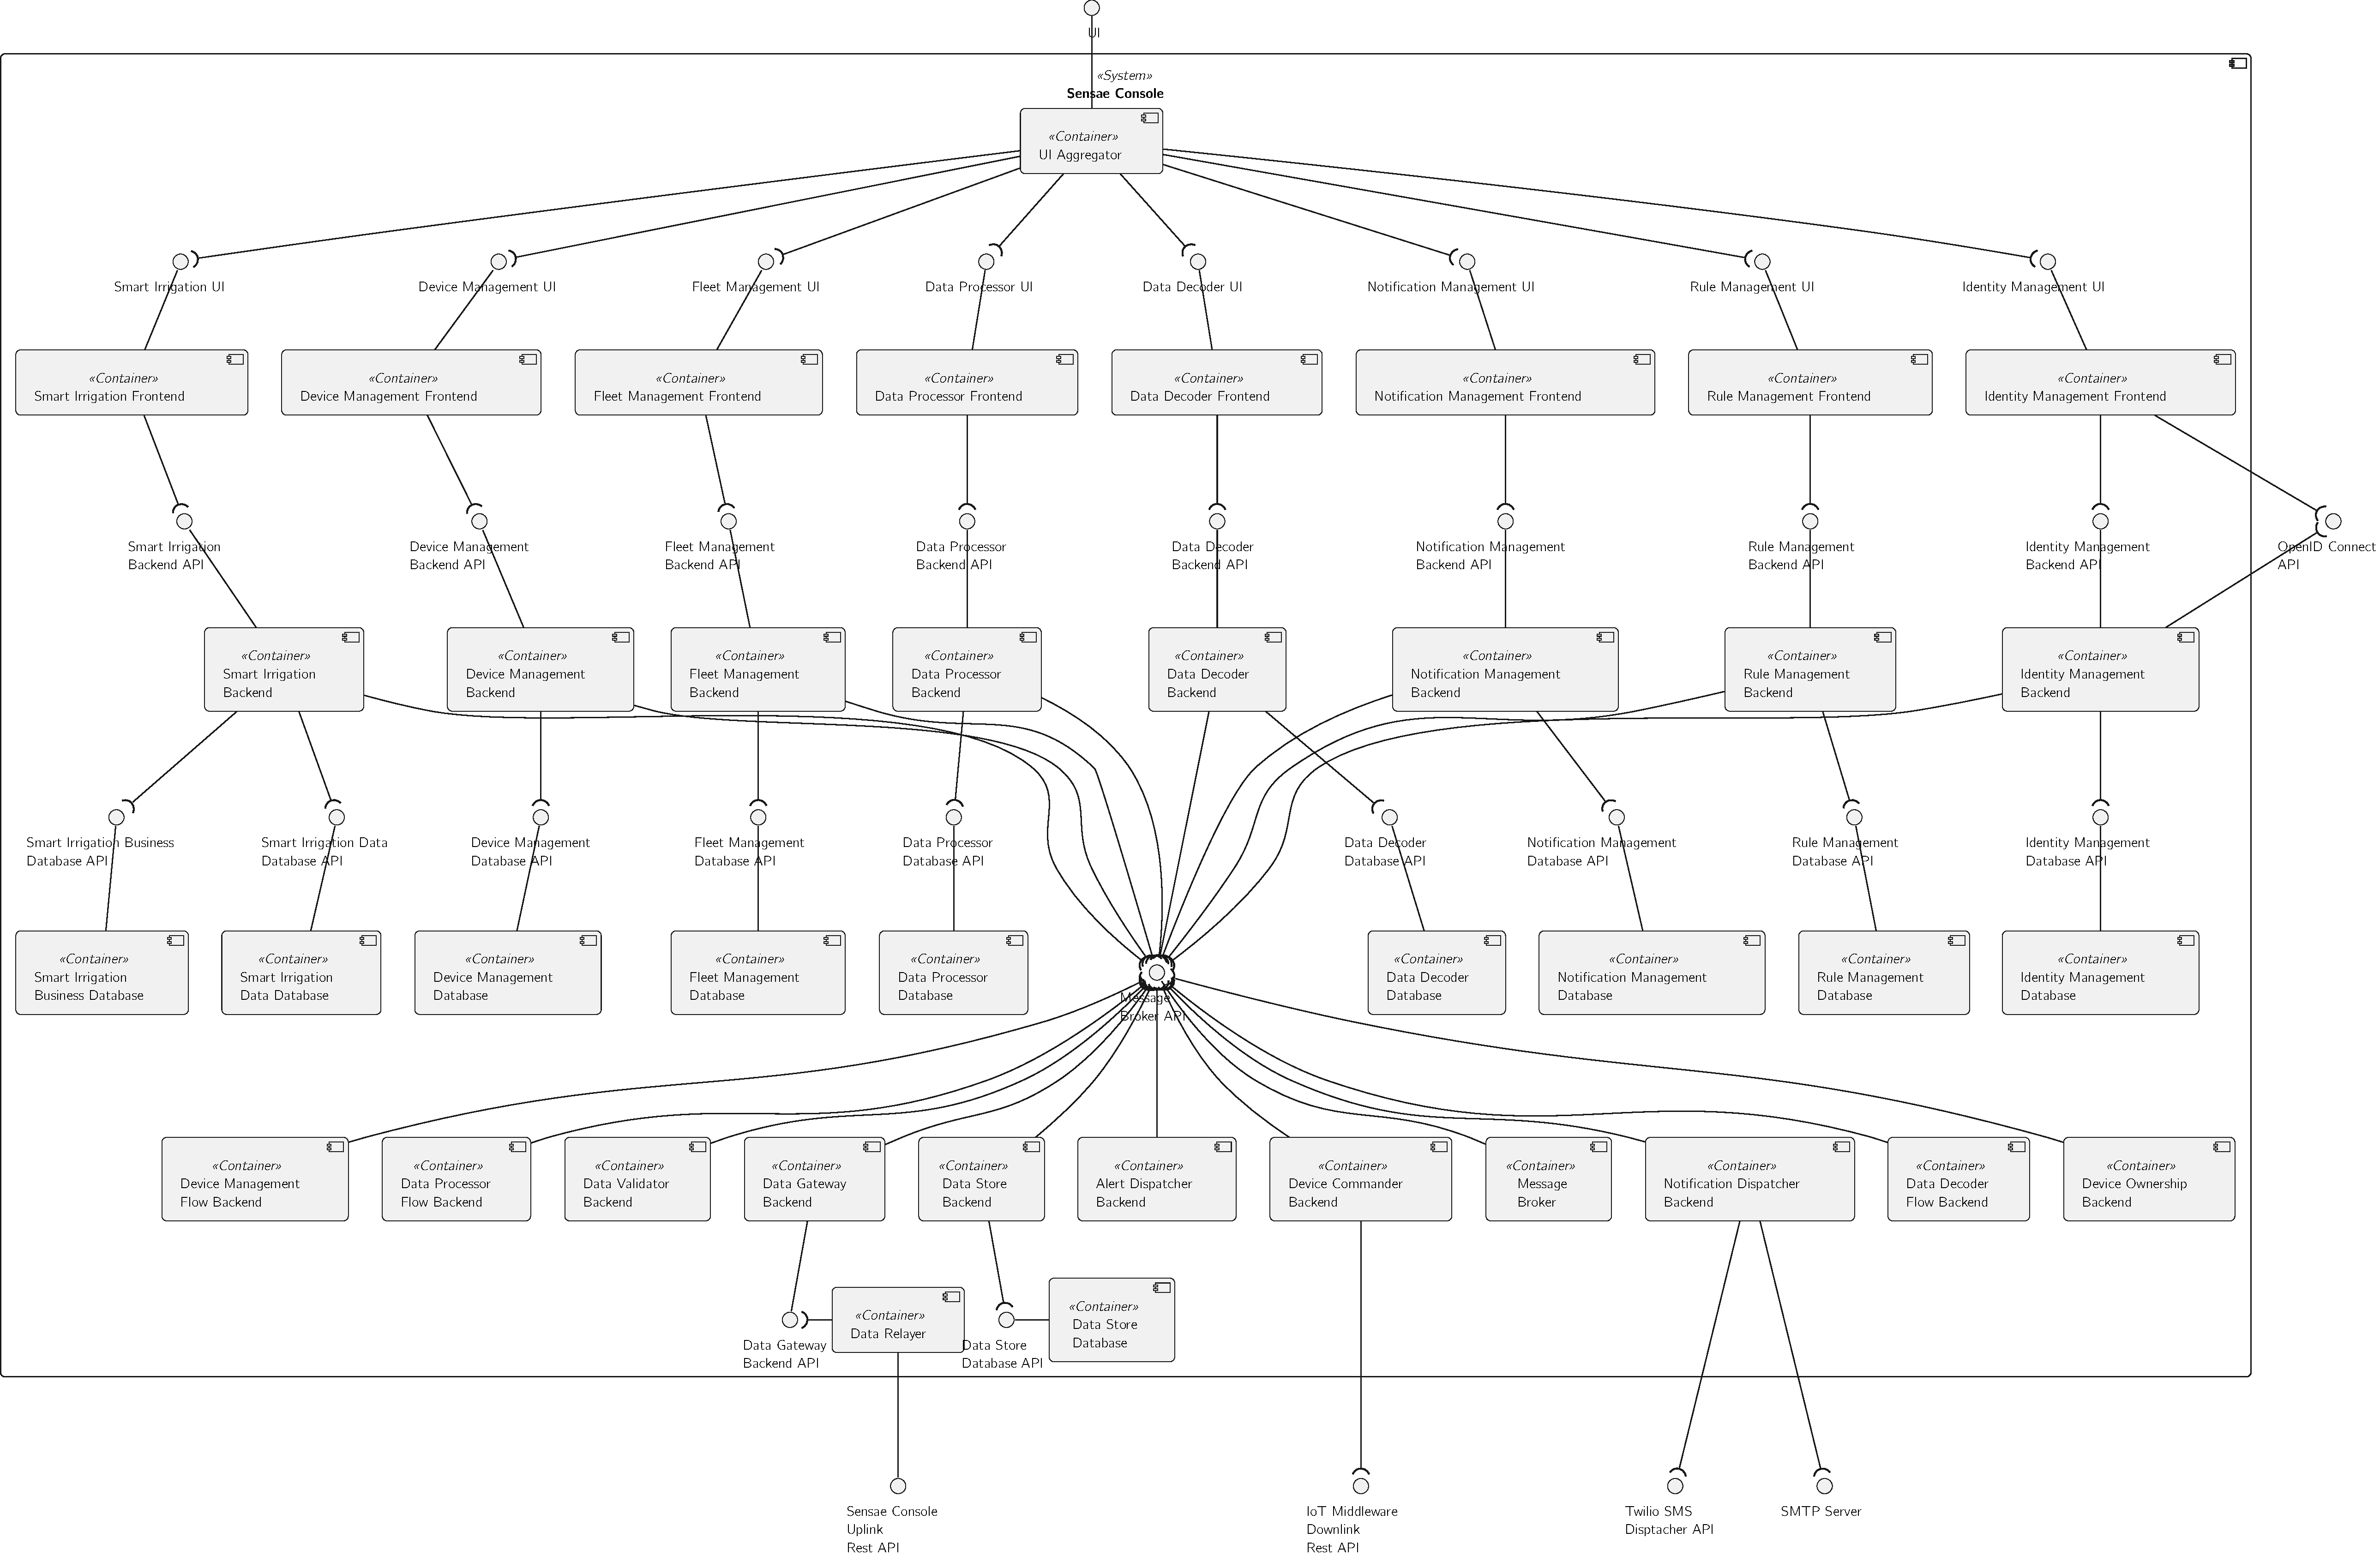
\includegraphics[page=1,width=0.8\columnwidth]{assets/diagrams/design/architectural/level2/logical/complete.pdf}
   \caption[Complete Solution - Container Level - Logical View Diagram]{Complete Solution - Container Level - Logical View Diagram}
   \label{fig:AppendixB:complete}
\end{sidewaysfigure}

%\chapter{Sensae Console - Components Level - Logical View}
\label{AppendixC}

This Appendix presents the logical view, component level, of the Data Flow scope containers that had minor differences when compared with the other containers.

\begin{figure}[H]
   \centering
   \resizebox{0.6\columnwidth}{!}
   {
      \input{assets/diagrams/design/architectural/level3/logical/data-gateway.latex}
   }
   \caption[Component Level - Data Gateway - Logical View Diagram]{Component Level - Data Gateway - Logical View Diagram}
   \label{fig:AppendixC:gateway}
\end{figure}

\begin{figure}[H]
   \centering
   \resizebox{0.6\columnwidth}{!}
   {
      \input{assets/diagrams/design/architectural/level3/logical/data-store.latex}
   }
   \caption[Component Level - Data Store - Logical View Diagram]{Component Level - Data Store - Logical View Diagram}
   \label{fig:AppendixC:store}
\end{figure}


\begin{figure}[H]
   \centering
   \resizebox{0.7\columnwidth}{!}
   {
      \input{assets/diagrams/design/architectural/level3/logical/device-commander.latex}
   }
   \caption[Component Level - Device Commander - Logical View Diagram]{Component Level - Device Commander - Logical View Diagram}
   \label{fig:AppendixC:commander}
\end{figure}


%----------------------------------------------------------------------------------------

\end{document}
